%!TEX root = presentazionelancia.tex
\section{The Data Model}

\begin{frame}
\frametitle{Tao Data Model}
 	T.A.O. stands for ``The Associations and Objects"
 	\begin{center}
 	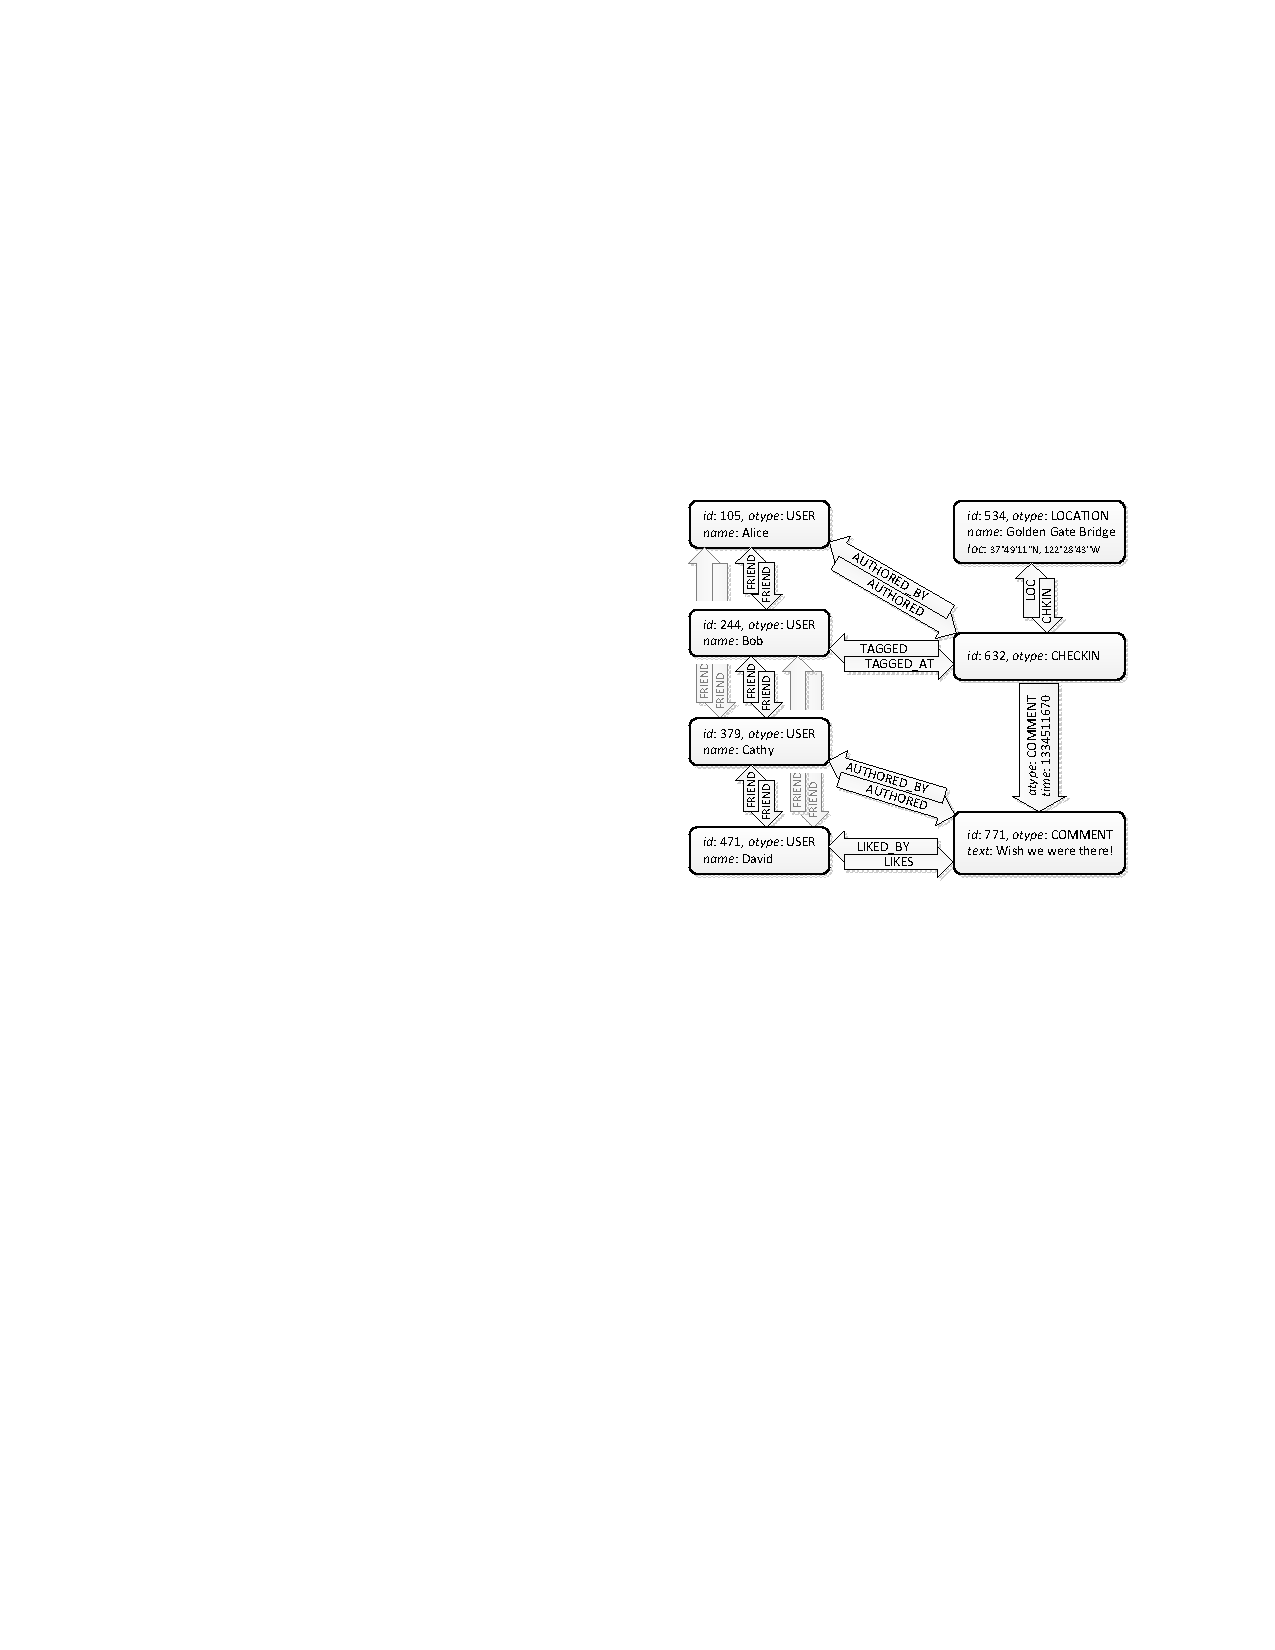
\includegraphics[width=0.6\textwidth]{figs/social2}		
 	\end{center}
\end{frame}

\begin{frame}[fragile]
\frametitle{Objects}
\onslide<1->
\begin{itemize}
	\item Typed nodes (type is denoted by \verb|otype|)
	\item Identified by 64-bit integers (unique) 
	\item Contains data in the form of key-value pairs
	\item Models users and repeatable actions (e.g. comments)
\end{itemize}
\onslide<2->
API for objects:
\begin{itemize}
	\item Allocate new object 
	\item retrieve
	\item update
	\item delete
\end{itemize}
\end{frame}


\begin{frame}[fragile]
\frametitle{Associations}
    \begin{itemize}
	\item Typed directed edges between objects (type is denoted by \verb!atype!)
	\item Identified by source object \verb!id1!, \verb!atype! and destination object \verb!id2!
	\item Contains data in the form of key-value pairs.
	\item Contains a 32-bit \verb!time! field.
	\item Models actions that happen at most once or records state transition (e.g. like)
	\item Often inverse association is also meaningful (eg like and liked by).
\end{itemize}
\end{frame}

\begin{frame}
\frametitle{Associations API}
\begin{itemize}
\item Add new
\item Delete
\item Change type
\end{itemize}
Also inverse association is created or modified automatically
\end{frame}

\begin{frame}[fragile]
\frametitle{Querying TAO}
TAO's associations queries are organized around \emph{associations~ list}

\begin{itemize}
\item \verb!assoc_get(id1,atype, id2set, high?, low?)!
\item \verb!assoc_count(id1,atype)!
\item \verb!assoc_range(id1, atype, pos, limit)!
\item \verb!assoc_time_range(id1,atype, high, low, limit)!
\end{itemize}

Query results are bounded to 6000 results
\end{frame}



